\documentclass[12pt]{article}
\usepackage{amsmath}
\usepackage{array}
\usepackage{cancel}
\usepackage[thinc]{esdiff}
% \usepackage{gensymb}
\usepackage{geometry}
\usepackage{graphicx}
\usepackage{pgfplots}
\usepackage{siunitx}
\usepackage{wrapfig}
\usepackage{xcolor}

\title{Homework \#9, 4B}
\author{Donald Aingworth IV}
\date{March 19, 2025}

\pgfplotsset{width=8cm,compat=1.9}
\usepgfplotslibrary{external}
% \tikzexternalize

\renewcommand\thesubsection{\alph{subsection}}
\newcommand{\proj}{\text{proj}}

\begin{document}

\DeclareSIUnit{\mile}{mi}
\DeclareSIUnit{\gal}{gal}
\DeclareSIUnit{\foot}{ft}
\DeclareSIUnit{\hour}{h}
\DeclareSIUnit{\rad}{rad}
\DeclareSIUnit{\unit}{u}
\DeclareSIUnit{\dyne}{dyn}

\maketitle

\pagebreak
\section{Problem 2}
\begin{wrapfigure}{r}{0.25\textwidth}
    \vspace{-30pt}
    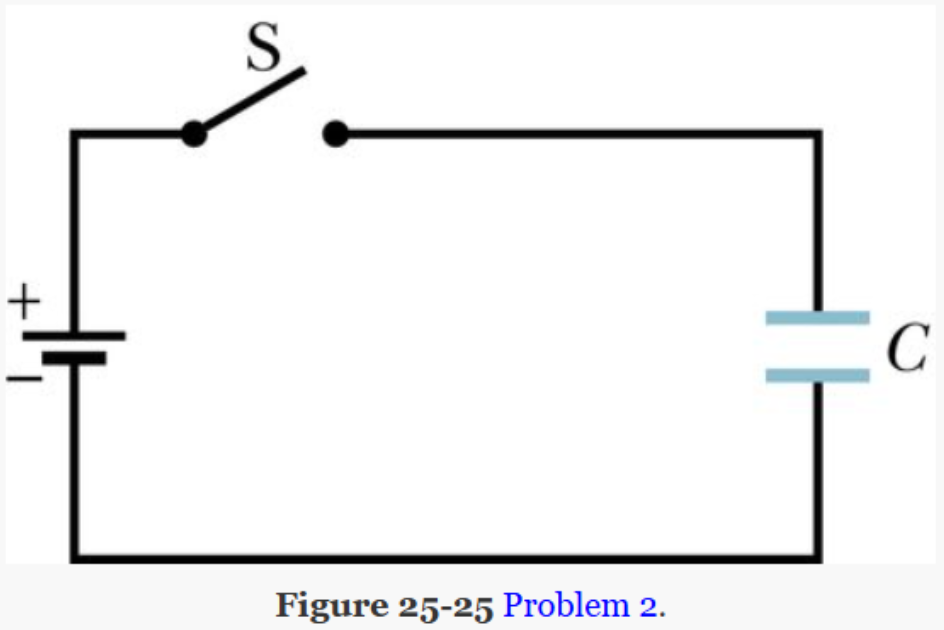
\includegraphics[width=0.25\textwidth]{picture_1.png} 
    % \label{fig:wrapfig}
\end{wrapfigure}
The capacitor in Fig. 25-25 has a capacitance of $25 \unit{\micro\farad}$ and is initially uncharged. 
The battery provides a potential difference of 120 V. 
After switch S is closed, how much charge will pass through it?

\subsection*{Solution: 3 mC}
We have an equation for this. 
For the capacitor to become fully charged, the charge that is the answer must pass into the capacitor and through the switch.
We have an equation for charge to enter a capacitor from voltage.
\begin{align*}
    q   &=  CV
        =   (25 \times 10^{-6}) * 120
        =   3000 \times 10^{-6} \unit{\coulomb}
        =   \boxed{\boxed{3 \unit{\milli\coulomb}}}
\end{align*}

\pagebreak
\section{Problem 4}
The plates of a spherical capacitor have radii 38.0 mm and 40.0 mm. 
(a) Calculate the capacitance. 
(b) What must be the plate area of a parallel-plate capacitor with the same plate separation and capacitance?

\subsection{Solution: 8.45 \texttimes\ 10$^{-11}$ F}
We have, from conference, the equation for the capacitance of a spherical capacitor.
We can use that to calculate the capacitance of our spherical capacitor.
\begin{align*}
    C   &=  4\pi\varepsilon_0 \frac{ab}{b - a}
        =   \frac{1}{8.99 \times 10^9} \frac{0.038 * 0.040}{0.040 - 0.038}\\
        &=  \frac{1}{8.99 \times 10^9} \frac{1.52 \times 10^{-3}}{2 \times 10^{-3}}
        =   \frac{0.76}{8.99 \times 10^9}\\
        &=  \boxed{8.45 \times 10^{-11} \unit{\farad}}
\end{align*}

\subsection{Solution: 191 cm$^2$}
The plate separation must be 2 \unit{\milli\meter} and the capacitance must be the above.
We have an equation that we can use for this.
\[
    C   =   \frac{\varepsilon_0 A}{d}
\]
\begin{align*}
    A   &=  \frac{Cd}{\varepsilon_0}
        =   \frac{8.45 \times 10^{-11} * 2 \times 10^{-3}}{8.85 \times 10^{-12}}\\
        &=  \frac{16.9}{8.85} \times 10^{-2} \unit{\meter^2}
        =   1.910 \times 10^{-2} \unit{\meter^2}\\
        &=  \boxed{191 \unit{\centi\meter^2}}
\end{align*}

\pagebreak
\section{Problem 5}
What is the capacitance of a drop that results when two mercury spheres, each of radius $R$ = 2.00 mm, merge?

\subsection*{Solution: 2.803 \texttimes\ 10$^{-13}$}
Mercury is a liquid at room temperature. 
The volume resultant would be equal to the volume of the two other spheres added together.
To avoid big numbers, we're just going to say that the small spheres will have radius $R$ and the big sphere will have radius $R'$. 
As such, we will find the value of $R'$.
\begin{gather*}
    V'  =   2V_0\\
    \frac{4}{3}\pi R'^3 =   2*\frac{4}{3}\pi R^3\\
    R'^3    =   2R^3\\
    R'      =   R\sqrt[3]{2}\\
    R'      =   0.002 * \sqrt[3]{2}
            =   2.520 \times 10^{-3} \unit{\meter}
\end{gather*}

From this, we can get the capacitance.
\begin{align*}
    C   &=  4\pi\varepsilon_0 R'
        =   \frac{2.520 \times 10^{-3}}{8.99 \times 10^9}
        =   \boxed{2.803 \times 10^{-13} \unit{\farad}}
\end{align*}

\pagebreak
\section{Problem 19}
% \begin{wrapfigure}{r}{0.4\textwidth}
%     \vspace{-30pt}
    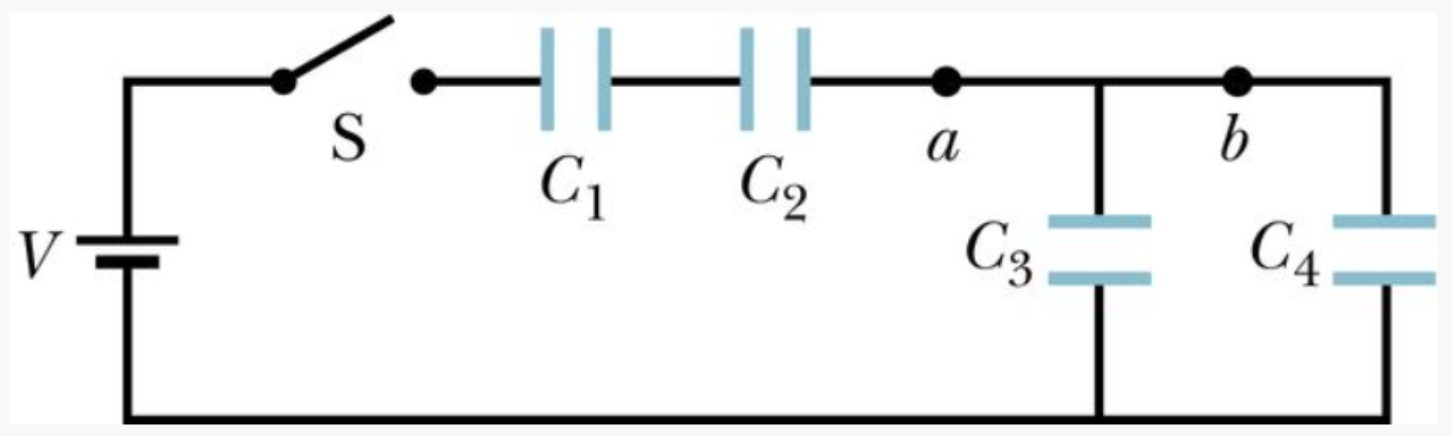
\includegraphics[width=\textwidth]{picture_4.png} 
%     % \label{fig:wrapfig}
% \end{wrapfigure}
In Fig. 25-34, the battery has potential difference $V = 9.0\unit{\volt}$, $C_2 = 3.0\unit{\micro\farad}$, $C_4 = 4.0\unit{\micro\farad}$, and all the capacitors are initially uncharged. 
When switch $S$ is closed, a total charge of $12 \unit{\micro\coulomb}$ passes through point $a$ and a total charge of $8.0 \unit{\micro\coulomb}$ passes through point $b$. 
What are (a) $C_1$ and (b) $C_3$?

\subsection{Solution: 4\textmu F}
Let's start by calculating $C_3$. 
Before the charge split, $12\unit{\micro\coulomb}$ of charge pass through the wire. 
It gets split, and $8\unit{\micro\coulomb}$ goes through the wire to $C_4$. 
The remaining $4\unit{\micro\coulomb}$ of charge has to go somewhere, so it goes through the wire to $C_3$.
Since electric potential difference is the same for each capacitor in parallel, we can create a formula for this.
\begin{align*}
    V_3 = V_4\\
    \frac{Q_3}{C_3} = \frac{Q_4}{C_4}\\
    \frac{C_3}{Q_3} = \frac{C_4}{Q_4}\\
    C_3 = \frac{Q_3}{Q_4}C_4
        &=  \frac{4}{8}*4 \unit{\micro\farad}
        =   \frac{4}{2} \unit{\micro\farad}
        =   2 \unit{\micro\farad}
\end{align*}

Now that we have $C_3$, we can use equivalence to find the capacitance of all capacitors together.
We know that the charge passing through any part of the circuit (not separated in parallel) is equal, and that charge must be $12\unit{\micro\coulomb}$.
We also know that the potential difference across the circuit must be the given potential difference of 9V. 
We can use this to calculate the capacitance across the circuit.
\[
    C_{\Sigma} = \frac{Q_0}{\Delta V} = \frac{12 \unit{\micro\coulomb}}{9 \unit{\volt}} = \frac{4}{3} \unit{\micro\farad}
\]

With this, we can set up a series of equations from capacitances in series and in parallel to find $C_1$.
\begin{align*}
    C_{34} = C_3 + C_4 &= 2 \unit{\micro\farad} + 4 \unit{\micro\farad} = 6 \unit{\micro\farad}\\
    \frac{1}{C_{\Sigma}} = \frac{1}{C_1} + \frac{1}{C_2} + \frac{1}{C_{34}}\\
    \frac{1}{C_1} = \frac{1}{C_{\Sigma}} - \frac{1}{C_1} - \frac{1}{C_2}
        &=  \frac{3}{4 \unit{\micro\farad}} - \frac{1}{3 \unit{\micro\farad}} - \frac{1}{6 \unit{\micro\farad}}
        =   \frac{9}{12 \unit{\micro\farad}} - \frac{4}{12 \unit{\micro\farad}} - \frac{2}{12 \unit{\micro\farad}}
        =   \frac{3}{12 \unit{\micro\farad}}\\
    C_1 &=  \boxed{4 \unit{\micro\farad}}
\end{align*}

\subsection{Solution: 2\textmu F}
We found it in part (a). It's \boxed{2\unit{\micro\farad}}.

\pagebreak
\section{Problem 22}
\begin{wrapfigure}{r}{0.4\textwidth}
    \vspace{-30pt}
    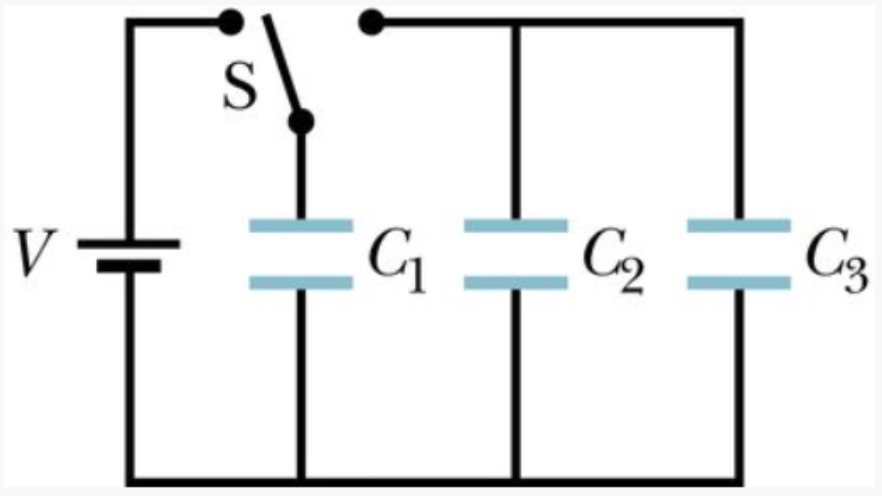
\includegraphics[width=0.4\textwidth]{picture_5.png} 
    % \label{fig:wrapfig}
\end{wrapfigure}
In Fig. 25-37, $V = 10 \unit{\volt}$, $C_1 = 10 \unit{\micro\farad}$, and $C_2 = C_3 = 20 \unit{\micro\farad}$. 
Switch S is first thrown to the left side until capacitor 1 reaches equilibrium. 
Then the switch is thrown to the right. 
When equilibrium is again reached, how much charge is on capacitor 1?

\subsection*{Solution: 20\textmu C}
Let's calculate the maximum charge on the capacitor $C_1$ , the charge it has when it gets released from the battery.
\begin{align*}
    Q   =   CV
        =   10\unit{\micro\farad}*10\unit{\volt}
        =   100\unit{\micro\coulomb}
\end{align*}

Now, when the capacitor is connected to the other two capacitors, it will have to share the capacitance with them.
For the sake of the problem, let's pretend that they are intead one capcitor, this time with charge $C_{23} = C_2 + C_3 = 40\unit{\micro\farad}$.
Since potential difference will be constant when we achieve equilibrium, we can have an equivalence here.
\begin{gather*}
    V_1 =   V_{23}\\
    Q   =   q_1 + q_{23} \rightarrow q_{23} = Q - q_{1}\\
    \frac{q_1}{C_1} =   \frac{q_{23}}{C_{23}}
        =   \frac{Q}{C_{23}} - \frac{q_1}{C_{23}}\\
    q_1 * \left( \frac{1}{C_1} + \frac{1}{C_{23}} \right)   =   \frac{Q}{C_{23}}\\
    q_1 =   \frac{Q}{C_{23}}*\left( \frac{1}{C_1} + \frac{1}{C_{23}} \right)^{-1}
\end{gather*}
\begin{align*}
    q_1 &=  \frac{100\unit{\micro\coulomb}}{40\unit{\micro\farad}}*\left( \frac{1}{10\unit{\micro\farad}} + \frac{1}{40\unit{\micro\farad}} \right)^{-1}\\
        &=  \frac{100\unit{\micro\coulomb}}{40\unit{\micro\farad}} * \frac{40\unit{\micro\farad}}{5}\\
        &=  \boxed{20\unit{\micro\coulomb}}
\end{align*}
This fits well with an idea that charge is given proportionally to the capacitance compared to the total capacitance, but that's a story for another day.

\pagebreak
\section{Problem 23}
\begin{wrapfigure}{r}{0.4\textwidth}
    \vspace{-30pt}
    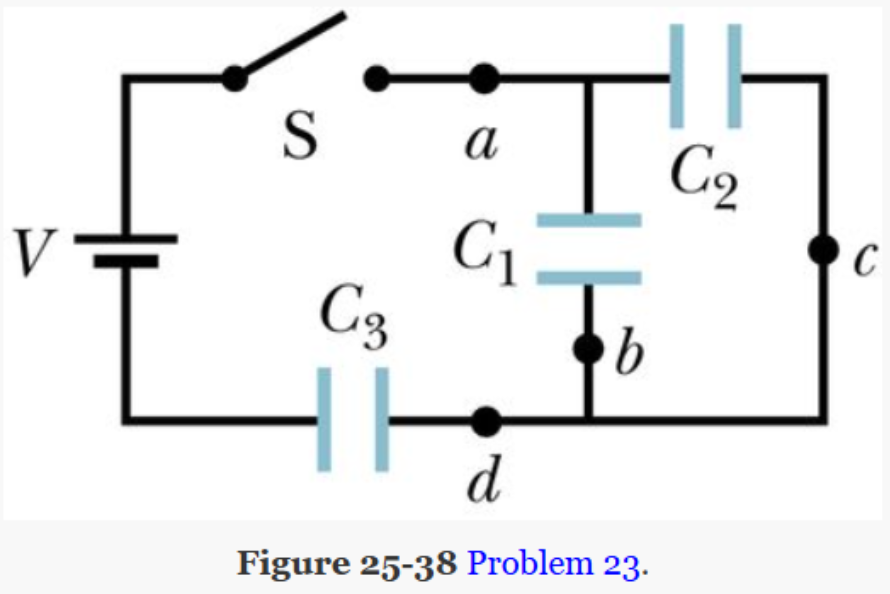
\includegraphics[width=0.4\textwidth]{picture_6.png} 
    % \label{fig:wrapfig}
\end{wrapfigure}
The capacitors in Fig. 25-38 are initially uncharged. 
The capacitances are $C_1 = 4.0 \unit{\micro\farad}$, $Cz = 8.0 \unit{\micro\farad}$, and $C3 = 12 \unit{\micro\farad}$, and the battery's potential difference is $V = 12 \unit{\volt}$. 
When switch S is closed, how many electrons travel through (a) point a, (b) point b, (c) point c, and (d) point d? 
In the figure, do the electrons travel up or down through (e) point b and (f) point c?

\pagebreak
\section{Problem 31}
A $2.0 \unit{\micro\farad}$ capacitor and a $4.0 \unit{\micro\farad}$ capacitor are connected in parallel across a 300 V potential difference.
Calculate the total energy stored in the capacitors.

\pagebreak
\section{Problem 32}
A parallel-plate air-filled capacitor having area $40\unit{\centi\meter^2}$ and plate spacing $1.0 \unit{\milli\meter}$ is charged to a potential difference of $600 \unit{\volt}$. 
Find (a) the capacitance, (b) the magnitude of the charge on each plate, (c) the stored energy, (d) the electric field between the plates, and (e) the energy density between the plates.

\pagebreak
\section{Problem 35}
Assume that a stationary electron is a point of charge. 
What is the energy density $u$ of its electric field at radial distances (a) r = 1.00 mm, (b) r = 1.00 um, (c) r = 1.00 nm, and (d) r = 1.00 pm? 
(e) What is $u$ in the limit as r → 0?

\pagebreak
\section{Problem 47}
A certain substance has a dielectric constant of $2.8$ and a dielectric strength of $18 \unit{\mega\volt/\meter}$. 
If it is used as the dielectric material in a parallel-plate capacitor, what minimum area should the plates of the capacitor have to obtain a capacitance of $7.0 \times 10^{-2} \unit{\micro\farad}$ and to ensure that the capacitor will be able to withstand a potential difference of $4.0 \unit{\kilo\volt}$?

\subsection*{Solution}


\end{document}